\documentclass[tikz]{standalone}
\usepackage{tikzducks, tikzlings, bearwear}

\begin{document}
    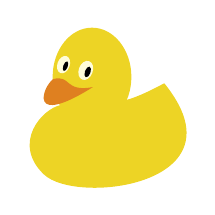
\begin{tikzpicture}
        \duck ;
    \end{tikzpicture}

    \definecolor{jacket}{HTML}{cc0c07}
    \definecolor{hat}{HTML}{d7c8c5}
    \definecolor{ribbon}{HTML}{381c1b}
    \definecolor{collar}{HTML}{000800}
    \begin{tikzpicture}
        \bear [
            strawhat=hat,
            ribbon=ribbon,
        ] \bearwear[
            shirt=jacket,
            body deco={
                \fill[ribbon] (node cs:name=beartummy, anchor=north) ++(-1cm, -0.07cm) rectangle ++(2cm, -0.1cm);
                \clip (node cs:name=beartummy, anchor=north) ++(-0.3cm, 0.6cm) rectangle ++(0.6cm, -1.2cm);
                \fill[collar] (node cs:name=beartummy, anchor=north) ++(0cm, 0.6cm) circle [radius=0.45cm];
            },
        ] ;
    \end{tikzpicture}

    \definecolor{jacket}{HTML}{3e2b19}
    \definecolor{head}{HTML}{000F0F}
    \definecolor{bill}{HTML}{30384f}
    \definecolor{eye}{HTML}{F0F0F0}
    \definecolor{neck}{HTML}{a8a296}
    \definecolor{feather}{HTML}{704b2b}
    \definecolor{underneck}{HTML}{F0F0F0}
    \begin{tikzpicture}
        \duck[
            laughing,
            body=neck,
            head=head,
            bill=bill,
            eye=eye,
            jacket=jacket,
        ] ;

        \begin{scope}
            \clip \duckpathjacket ;
            \foreach \x in {0.1, 0.4, ..., 2.2}
                \foreach \y in {0.2, 0.6, ..., 1.5}
                    \draw[feather, line width=1pt] (\x, \y) [
                        start angle=135,
                        end angle=255,
                        x radius=0.20,
                        y radius=0.10,
                    ] arc ;
            \foreach \x in {0.2, 0.5, ..., 2.2}
                \foreach \y in {0.4, 0.8, ..., 1.5}
                    \draw[feather, line width=1pt] (\x, \y) [
                        start angle=135,
                        end angle=255,
                        x radius=0.20,
                        y radius=0.10,
                    ] arc ;
        \end{scope}

        \begin{scope}
            \clip (0.90, 1.50) ellipse [x radius=0.50, y radius=0.625] ;
            \clip (0.40, 1.40) --
                  (1.40, 1.60) --
                  (1.40, 0.00) --
                  (0.40, 0.00) --
                  cycle
            ;

            \fill[underneck] (0.90, 1.525) ellipse [
                rotate=30,
                x radius=0.600,
                y radius=0.500,
            ] ;
            \fill[head] (0.90, 1.525) ellipse [
                rotate=30,
                x radius=0.600,
                y radius=0.300,
            ] ;
        \end{scope}

        %% Redraw eyes and bill on top of the neck
        \fill[eye, rotate=-20] (0.23,1.7675) ellipse [x radius=0.0893, y radius=0.125] ;
        \fill[black, rotate=-20] (0.26,1.7575) ellipse [x radius=0.0357, y radius=0.0714] ;
        \fill[eye, rotate=-20] (-0.06,1.74) ellipse [x radius=0.0786, y radius=0.1143] ;
        \fill[black, rotate=-20] (-0.03,1.73) ellipse [x radius=0.0286, y radius=0.0643] ;
        \fill[bill!80!black,overlay] (0.40,1.20) .. controls (0.54,1.36) and (0.65,1.31) .. (0.91,1.37) .. controls (0.45,1.06) and (0.36,1.18) .. (0.40,1.20) -- cycle;
        \fill[bill,overlay] (0.41,1.47) .. controls (0.64,1.53) and (0.54,1.30) .. (0.91,1.37) .. controls (-0.02,1.10) and (0.28,1.37) .. (0.41,1.47) -- cycle;
    \end{tikzpicture}
\end{document}
